\fancyhead[R]{{\scriptsize {\faBook\ }我们最幸福 > 应许之地}}%偶數頁眉的右邊
\chapter*{18 > 应许之地}
\addcontentsline{toc}{chapter}{\hspace{5mm}18 \textbf{>}\ \ 应许之地}
\vspace{10mm}
\begin{flushright}
	\textcolor{PinYinColor}{\EN \huge{The\\
			Promised Land\\
			\ \\}}
\end{flushright}

\begin{figure}[!htbp]
	\centering
	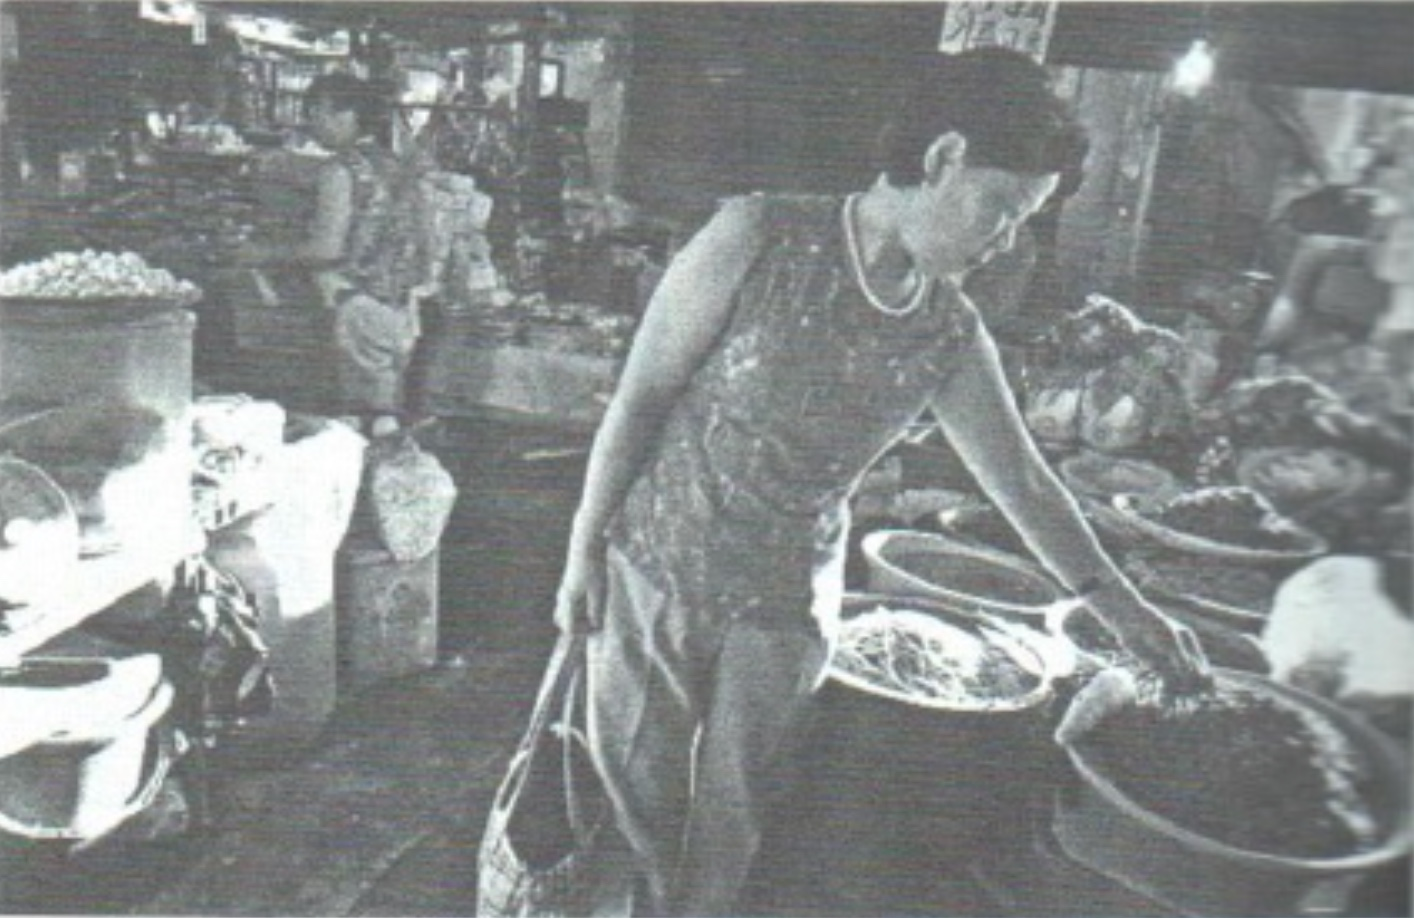
\includegraphics[width=6cm]{./Chapters/Images/18.jpg}
	\caption*{2004年宋女士在首尔的一个市场}
\end{figure}

2002年8月末,一个周二的早上,宋女士登上了韩亚航空从大连飞往南韩仁川国际机场的班机。此次旅行她用的是一个假名,拿着一本伪造的护照。她只认识同机的另一个人──坐在几排之外的一个年轻男子。他早上六点到了宾馆房间,给了她这本护照,那是从一个差不多年纪的南韩妇女那里偷来的护照,原来的照片被小心的用刀片取出,换上了宋女士的照片。如果被询问,她要说她是一个南韩游客,从韩国越过黄海,来大连一个海边度假村度长周末。为了看上去和掩人耳目的故事相符,宋女士全身上下穿着在北朝鲜会被认为是奇装异服的新衣服──紧身的牛仔裤,亮白的运动鞋,背着个运动背包。她的耳朵打了耳洞\footnote{一般北朝鲜妇女是没有耳洞的。}、头发剪短了并被烫成了她这个年纪南韩女人流行的式样。她还花了两个礼拜在中国增胖、打扮,让她看上去不至于像个难民。唯一会暴露身份的就是她的北朝鲜口音。因此她被建议尽量少说话。为了避免同邻座的乘客讲话,她被告知在接下来八十分钟的飞行里就待在自己的座位上。

她坐着一声不吭,手放在膝盖上。她不像想象中的一个人在此情形中可能会的那么紧张。她的沉着来自于自己确定现在所做的事情是正确的。她对于自己叛逃的决定感到平静。在农舍里听见电饭煲声音的那个早上,她所有的疑惑都烟消云散了。她已经答应接受玉熙去南韩的邀请。她想亲眼看看在电视上所看到的那个世界。她的女儿,她的孙儿女们有他们的机会──北朝鲜的形势不可能永远持续──但是她没有多少时间了。她要抓住这次的机会,但是首先她想回一趟清津同女儿们道个别。她想同她们解释下原因,再把玉熙在中国留给她的,差不多一千美元的钱分给她们。“我不能让你妹妹以为我死了。”她告诉玉熙。玉熙反对这个决定,她担心一旦回到家,她母亲会失去勇气或者妹妹们会劝阻她,但是她却非常坚持。

因为雨季,图们江水位上涨,她在清津待了差不多一个月;然而宋女士对自己的决定却没有动摇。她不达目的不罢休的信念支撑着她经历叛逃中最危险的时刻。玉熙雇佣的那个中间人也非常讶异的看到,这么个个子小小、和蔼可亲的阿婆,能够拿着假护照大气不喘的登上国际航班。

从中国出境和登机是此行最危险的部分。一旦中国出入境当局发现她的假护照,她就会被立即逮捕,并被遣送回北朝鲜,面临她的就是劳动营。现在,在飞机降落至南韩之后只有一个难关。她的护照不足以糊弄南韩人,在例行的检查中,他们很快就会发现这是一本被盗的护照。事实上,同机的那个年轻人在飞机降落之前就会收回这本护照,并且消失在人群之中。

“假装不认识我。”他告诉她。她要待在女厕所里,直到他安全的出了机场。然后她就径直走去移民柜台,说出真相。

她叫宋熙锡、五十七岁、来自清津。她在饥荒中失去了半个家庭,现在来南韩寻求自己和女儿的新生活。没什么好隐瞒的了。

按照南韩宪法第三条款规定,南韩将其视为半岛唯一的合法政府,这也就意味着半岛的所有人口,包括北朝鲜人,将自动成为其公民。北朝鲜人成为南韩公民的权利在1996年被高等法院所支持。然而,现实却复杂的多。为了拿到公民权,北朝鲜人必须自行抵达南韩。一个北朝鲜人不能在南韩驻北京大使馆或者其它各地的领事馆主张公民权。基于残存的一点对其共产主义盟友的忠诚,以及对数以百万计的北朝鲜人可能越境的担忧,中国不允许庇护寻求者出现在这些外交场所。中国人知道大批东德叛逃者于1989年逃至匈牙利和捷克斯洛伐克。迫使当局开放柏林墙,而东德政府也随之垮台。

南韩政府也尽力将收容的难民数量压低至一个可控的水平。潮水般的脱北者来到南方将带来极大的财政和社会负担。

那些设法进入南韩的人所用的方式也是五花八门。如果他们有钱或者有关系,他们会弄到假护照,飞往南韩。或者,他们会从逃出中国,到其邻国如蒙古或者越南,在那里的南韩大使馆对于接收脱北者还不是很限制。还有一小部分是闯入欧洲国家驻中国大使馆或者联合国驻中国办公机构,并寻求庇护。

在中国的十万或者更多北朝鲜人只有很少一部分想方设法到了南韩。在1998年只有七十一名北朝鲜人要求南韩公民资格;1999年这个数字上升到了一百八十四名;2000年有三百一十二名;2001年有五百八十三名。到了2002年多达一千一百三十九名北朝鲜人被接纳。在此之后,人数就一般稳定在每年一千至三千人之间。

到宋女士到达的时候,南韩官员已经对机场里突然出现没有任何身份文件的北朝鲜人习以为常了。她到达仁川机场只引起了一阵忙碌,而没有恐慌。

下了飞机后的头几分钟里,宋女士都分不清东南西北。她之前只到过一次机场──那就是那天早上在中国登机的时候──而且那个和这个完全不同。耗资五十五亿美元的仁川机场一年前刚刚落成启用,机场距1950年道格拉斯·麦克阿瑟(Douglas MacArthur)将军登陆的地点不远。作为世界上最大的机场之一,它是一个玻璃和钢架的庞然大物。阳光穿过玻璃,照射着长长的抵达走廊。人们毫不费力由各个到达口前面的自动电梯运送着。宋女士不知道要去哪里,所以她就跟着其它的乘客同时又与那个护送的男子保持一定的距离。当其它的乘客在移民局柜台前排起长龙的时候,她躲进了女卫生间,在里面她发现那里同机场其它的地方一样让她不知所措。她不知道怎么让马桶冲水。洗脸盆上的水龙头是自动开关的,不用接触。她把头探出卫生间看看那个男的走没有,但是她从后面看见他还在排队,所以她又缩了回去。她又重新整理了下头发,补了补妆,看见镜子里一个不太熟悉的脸正盯回自己。

第二次,她看的时候,他已经走了。她壮了壮胆,从卫生间出来,想找个警官。她差点撞上一个很高的男人,他的徽章、名卡和宋女士的眼睛一般高。她深深的鞠了一躬,就像恳求一个官老爷一样,然后按照事先安排的那样说。

“我来自北朝鲜。我在这里寻求庇护。”她说。

这个人是个警卫。他看上去被吓了一跳,但是他知道该做什么。

“你一行几人?”他问道,一般脱北者都是集体抵达。她告诉他,就她一人。他领着她到了移民柜台傍边的一个办公室。打了几个电话,几分钟之内来了一些从国家情报局NIS的探员\footnote{NIS是南韩类似于美国中情局CIA的机构。}。

对宋女士的审讯持续了近一个月。之后她被转移到了位于机场附近的一个由NIS设立的专门收容新到脱北者的住所。她不允许离开那里,但是玉熙可以来看她。NIS的第一个工作是确定宋女士既不是间谍也不是诈降,以作为北朝鲜特工的卧底,任务是监视那些多年前被捕叛变的叛逃者。NIS还要筛除那些中国籍朝鲜人,他们冒充北朝鲜人,要求获得南韩公民资格,以及领取价值两万美元的安家费用。宋女士每天早上进行两个小时的谈话,然后把所谈内容写下来。她被要求把清津的主要地标标记出来──劳动党办公室、书记办公室、里和洞的边界\footnote{里(Guo)和洞(Dong)是朝鲜一级行政单位,相当于中国的乡和村。──译者},即地区和邻里的边界,北朝鲜人按这种方式被组织起来。她发现她很喜欢这种谈话:他们给了她一个反思自己生活的机会。在下午,她就会打个盹,再看看电视。那里有个小细节让她很开心──冰箱里堆满了免费的果汁,每个都独立包装带有吸管。

她后来回忆在NIS的日子,那是她生命里的第一次假期。在那之后,艰苦的工作又开始了。

对于每天只赚取一美元的人来说,要融入世界第十三大经济体绝非易事。南韩的人均收入大概在两万美元每年,是北朝鲜的十四至五十倍。

非军事区两边大量的宣传都致力于宣传北、南朝鲜人是怎么的一样。Hannar,同一个民族、同一个国家。但是六十年的分离使得他们之间又是如此不同。南韩是世界上科技最发达的国家之一。然而,大多数的北朝鲜人根本不知道因特网的存在,南韩家庭宽带网络的覆盖率比美国、日本和大多数欧洲国家都高。北朝鲜的文化、经济水平却仍然停留在上个世纪的水平。他们的语言也不再一样;南韩的版本现在大量的借用英语。身体上也是,双方的差别越来越大。由于大量食用牛奶和汉堡,南韩十七岁男性平均身高比他们北朝鲜的同龄人高出十五公分。北朝鲜人的语言及饮食和南韩在六十年代类似。

随着脱北者人数在九十年代节节攀升,南韩政府对他们能否成功融入社会的忧虑也持续增长。这个国家的智库分成不同的小组包括心理学家和社会学家,历史学家和教育家提出了一个计划。虽然脱北者数量不大\footnote{截至2008年末,总计四千四百万人口中,有一万五千零五十七名脱北者。},然而某天当南北统一之时,这个数字可能是成百万。“如果这个数量相对很小的脱北者群体不能适应,那么我们统一的前景就很暗淡。”一位涉及此项研究的南韩社会学家,尹麟镇(Yoon In-jin)说道。“如果他们能够成功的在这里开始新生活,我们就有希望融合。就此而言,我们不得不努力帮助他们,这样我们就可以从对他们的实验中吸取经验和教训。”

这些南韩学者研究了很多历史模式。他们参观了以色列为来自前苏联和北非的新抵达的犹太人设立的学校,这些人行使了他们回归犹太国家的权利,但是却对它的语言、文化知之甚少。他们也研究了在统一后德国里的东德人如何调整他们的生活。

1999年,他们在首尔以南八十公里的一个僻静的园区里设立了名为统一院(Hanawon)的临时难民所。那是兼具培训学校和进入社会前的过渡之所功能的一个机构,这个中心教授北朝鲜人如何靠自己在南韩生活。他们教授如果使用自动贩卖机、如何付电子账单。他们还教罗马字母,使他们可以阅读夹杂一些英文的广告。北朝鲜人还要从脑中剔除他们先前被灌输的东西──关于朝鲜战争和美国在二战中的角色。脱北者还要上关于人权的课程和学习民主机制。

在教室里,一切看上去都合乎情理,但是一旦到了统一院外面,宋女士就变得超级困惑。她的课程里有买衣服的现场实践。他们剪了头发。他们去饭店,那里每个人付钱买自己的午餐。然而他们都买了面条;没人闹得明白其它食品到底是什么。

有时候宋女士离开园区,外面喧闹的简直要让她晕过去。太吵闹了,到处都是灯光,让她目不暇接。她的眼睛流连于建筑物上那些生机勃勃的巨大荧光屏之间──有些有五米高──都是宽荧幕。但是大多数播放的东西她都不明白。什么HDTV、MTV、MP3、MP4、XP、TGIF、BBQ──看上去像个代码,不明白什么意思。但是让她最感到最神秘的还是人们自身。她知道他们都是朝鲜人,但是怎么他们看上去完全像另外一个种族。女孩们穿着那么短的裙子和真皮的长筒靴。很多人还染了发──男男女女都有,有红的、有黄的,就像洋人一样。他们耳朵上都戴着一个塑料的塞子,还有电线连到他们的口袋里。最震撼的还是,男孩、女孩手挽手的走在大街上,甚至还会当众相互亲吻。宋女士赶紧左右看看,但是没人注意他们。有一天,她去首尔的一个地铁站,在哪里她看见人潮乘着扶梯,沿着走道行进,在不同的线路之间换乘。她很惊奇于他们是怎么知道该往哪儿走啊。

宋女士在统一院待了三个月。在居住期的最后,还有个毕业典礼。后来,她被给了两万美元的安置费用开始新生活。之后,她就要靠自己了。

当我2004年遇见宋女士的时候,她已经离开北朝鲜两年了。当时,我正在为《洛杉矶时报》(Los Angeles Times)采访来自清津的人。我们安排在首尔的档案馆里见面。我在门口欢迎她,她穿着得体、个子很小、浑身散发着自信。她戴了一个很大的玉戒指,粉红Polo衬衣的下摆整洁的扎进米黄的裤子里。她身上的一切,从令人愉悦的清淡色彩到精心做的头发,都揭示这是个生活顺心如意的女人。

在离开统一院之后,宋女士找了份保姆的工作。她习惯于在北朝鲜的全日制工作,因此在全新的生活里,如果闲在家,她会很压抑。她决定不和玉熙生活,而是有个自己的公寓,并且在水原市的一个大楼里租了个工作室,水原位于首尔以南三十二公里,那里的租金比较便宜。生活上节俭一些,加上不断的工作,她很快就负担的起旅游的费用──这可是以前做梦都不敢想的事情。她加入了那种专门针对年长者并提供餐饮的旅游团,逛遍了南韩的每个角落。她甚至还回了趟中国──这次是作为观光客。她也随着一个去人权大会上发言的脱北者团体去了波兰。她交了很多朋友。她甚至还开始约会。她喜欢逛市场,尝试各种新鲜东西──芒果、猕猴桃、木瓜。她很喜欢在外吃饭。但是她还是培养不来吃披萨饼或汉堡包的胃口,但是她爱上了南韩式在桌子上烤的牛肉、猪肉。

大概每六个月,宋女士和我就要聚一下,吃顿饭。当我写关于北朝鲜的文章时,我发现她成为我特别可信的评论者。她从不为北朝鲜政权辩护──“那帮腐朽的混蛋!”她有一次提到金正日的时候这么说,这是是我唯一一次听见她嘴里冒出不敬的字眼──但是她和我遇到的其它遭受苦难的脱北者不同。她还怀念着关于北朝鲜的一些──邻里之间的友情;崩溃之前的免费医疗保障。她怀念年轻时刚结婚的那段日子。每次谈到她前夫,她的眼睛会湿润,她的圆脸也会温柔。

“当我看着眼前这些好吃的,就会让我流眼泪。”一天晚上,当我们围坐在一起吃涮牛肉(Shabu-Shabu)的时候,涮牛肉就是把切成薄片的牛肉放进清汤里煮熟后蘸着芝麻酱吃,宋女士这样道着歉。“我禁不住想起长博最后的话,‘让我们去好点的馆子,点瓶好的红酒。’”

当话题来到她儿子的时候,她就泣不成声,完全开不了口。如果我提起这个话题,她会移开她的目光。玉熙后来告诉我,她母亲永远不能原谅自己反对他爱上年长的女人,并且她不能设法让他活下来。

但是那都是过去的事情了,也是宋女士不愿详述的记忆。现在她能好好的品位自由和安度剩余时光。她对很多的事情都好奇。“我觉得我现在越活越年轻,也更大胆了。”她告诉我。当我问她很多关于北朝鲜的问题时,她也几乎问了我同样多关于美国和其它我去过地方的问题。每次我们的约会,她都是充满激情活力的出现,总是穿着崭新的、明快的、愉悦的套装。在多年的为他人牺牲之后,现在她开始为自己着想了。她甚至还长出了小肚子──这让她大吃一惊,这么多年的匮乏之后还能长胖──她开始节食了。她总是化妆。有一次,我坐火车去水原碰她,我们穿过拥挤的候车室相互看见。一旦我们走近到说话可以相互听见的距离,她就叫出来了,再也掩饰不住她的兴奋。“看看我,我做了眼睛!”

她去做了美容手术,在眼睑上加了双眼皮使得她看上去更像白种人的眼睛。这在南韩非常流行。宋女士完全融入了。

一心想着逃离的玉熙却不如她母亲在南韩生活的那么快乐。玉熙是个更容易惹麻烦的人,很快发现自己又有麻烦了。母女两在一起时,总会让人惊奇:一样的心形的脸型,一样的小小个头,但是他们的个性却又是如此之不同。玉熙总是穿黑色──黑牛仔裤、发亮的黑衬衣、黑色高跟靴子。带着多角的那种金属边眼镜而且修了眉,给人感觉不苟言笑。宋女士和女儿感情很好,一见面总是相互抚摸着头发和拥抱,就好像她们刚刚团聚一样,但是她们仍然会就政治话题斗嘴。吃完午饭,我的一个在援助机构工作的朋友问她们是否认为人道主义救援能否抵达那些预想接受对象的手中。玉熙认为那些援助都被抽调去给军队和党干部,加强金正日对北朝鲜的控制。

“但是如果那也能救些生命……”宋女士说。

玉熙打断她。“你在替邪恶政权说话。”

宋女士把嘴抿成了一条直线且在接下来的吃饭时间里不太说话了。

玉熙看上去总是笼罩在怨恨之中。自从她来到南韩,她一直被钱的问题困扰,事实上甚至在她离开中国之前就有了。她总是身处一些底层的中国人和韩国人之中,那些人生活在靠伪造、走私和放高利贷过活的阴暗世界。而且,通常他们还贩卖人口。他们将妇女偷运过河,进入中国,然后他们用偷来的护照将一些人弄进南韩。当玉熙最后一次离开北朝鲜,她没钱让自己从中国去南韩。一个走私贩同意给她一本护照和飞机票,作为回报,她则要从南韩政府支付给她的安家费中拿出一万四千美元给他。他们签署了协议,因为无从知晓相互的真实姓名,他们按了手印。

从统一院出来的一个星期后,这个走私贩的电话就打到了玉熙的手机上。她刚刚才买的手机──通常手机不可避免都是脱北者首先买的东西──她怎么也想不通那些人是怎么找到她,并弄到她的号码。他坚持她要马上付钱。

“我在首尔。我会在你公寓门口等你。”他告诉她。

玉熙很惊慌。安家费比预想的要少。二十多岁、三十多岁脱北者的安家费比年长的人要少,因为他们被认为可以去工作。她已经付了三千美元的押金租公寓。她同意在警局门口见这个走私贩。在经过长时间的讨价还价之后,她终于让对方同意降低收费,八千美元,差不多是她剩下的所有钱。

在那之后,玉熙在殡仪馆找了份工作,希望籍此能让自己的经济状况回到正轨。她可能已经做到了,如果不是陷入了深深的思念。

她想妈妈。一直以来,玉熙都有着一个念头,把妈妈也带过来,在到了南韩之后,这个念头就变得愈发的强烈。她自己也很吃惊的发现,在这里年长者能得到多么好的对待。

“在北朝鲜,当你太老不能工作的时候,没人会想要你。”她说。“他们恨不得把你一脚踢开。在南韩,我看见老人在唱歌、跳舞。我想到我的母亲,她辛勤工作了一辈子。我想她应当过的轻松一点。”

知道宋女士不容易被说服离开北朝鲜,于是玉熙又求助于同一伙人。在一起,他们制定了计划诱使宋女士跨境到中国。玉熙很担心如果什么地方出了岔子,母亲会被关进劳动营,而且希望母亲用最安全、最不可怕的线路。整个叛逃被安排的像个包价旅行,而且宋女士走的是头等舱。她的打包服务包括私人汽车载宋女士从清津去边境,买通北朝鲜边境警卫送她过河,及一本偷来的南韩护照。“我可以选择更便宜的。”玉熙解释,“但是,我想让她像个贵宾一样的来。”

玉熙因此也深深陷入债务泥潭。她签约殡仪馆做额外的工时,但是加班也不足以偿清债务。她又想其它的法子赚钱。她已经是个三十八岁的妇女,唯一的专业技能就是勉励人们为了金日成而努力工作──这在南韩可是鲜有市场。

她转向Karaoke的生意。他们叫Noribang,字面意思就是唱歌房,是用来让客人,通常是男性客人,放松唱歌的地方。俱乐部里有私人包间,里面有音响系统、麦克风、视频屏幕、软饮料和小吃。然而,真正吸引人的是女招待,她们可以陪唱、陪跳、陪酒甚至可以吃点豆腐──或者再多一点。在这种娱乐场所,玉熙的角色就是招募年轻女性,带她们出入俱乐部,确保她们不与顾客惹上麻烦。她的地盘就在水原周边。大部分来Karaoke的客人都是建筑工人,他们住在临时工棚里,晚上没什么娱乐。玉熙手下有二十个姑娘,她们都是北朝鲜人。她们大部分都是二十出头,一出统一院就被招入。

“她们来到南韩,没什么技能。”玉熙解释。“他们很快就知道,在办公室或者工厂做,一个月赚个九百美元。而这里,她们一晚上就可以赚一百美元。”有一天晚上,当我陪着她们到处转的时候,玉熙解释道。当时,她正开着一部现代面包车,车厢地板上满是揉瘪的香烟盒和赞美诗的盒式录音带。时间是下午五点,玉熙刚刚开始一天的工作。她随着下班高峰的车流出了水原城,然后下了高速,开上了一条两边布满田地和温室的两车道小路。之后路旁出现个小镇,她停下车,接了个女人上车,她看上去像个女学生的装扮,穿着鞋跟像钉子一样尖的凉鞋。虽然,在警方看来,她的工作是非法的,但是玉熙坚称她的女孩不是妓女。“我不强迫她们做什么。我告诉她们,你所要做的就是唱歌和跳舞,再从客人那里弄些钱。”这里的生意比在大城市好做些。“在首尔,她们要做的比这儿多。在首尔,那些穿西装的男人付钱喝酒,然后他们还总是期待着从姑娘那沾点便宜。这里的建筑工人虽然粗鲁些,但是很幼稚。”

这份工作给玉熙带来不错的收入,因此她也有足够钱以一万美元一个的价格,将她的两个妹妹都带来南韩。她最小的妹妹还把五岁的女儿带来了。而二妹则把丈夫和两个儿子都带来了。现在姐妹几个都在做Karaoke的生意。

玉熙唯一带不出来的家庭成员就是她的挚爱──自己的孩子。对此,她深怀负罪感。“我为了自己的自由,牺牲了我的孩子。”她这样自责道。我最后一次遇见她是2007年的夏天;她的儿子现在已经十八岁了,女儿也十六岁了。然而自从1998年在清津,当她穿着睡衣从家庭出走之后,她就再也没有见到过他们。虽然,她会定期的通过在中国的中间人给他们送钱,这些中间人收取佣金,然后再偷偷的越过边境把钱送进北朝鲜。她离开北朝鲜后不久,在北朝鲜边境离中国足够近,以至于可以扑捉到中国的移动电话信号的城市里,开始有非法的电话服务。因此,玉熙每隔几个月就能同她分居的丈夫通话。他会去茂山,用一个偷运进去的中国的手机,但是他不许她同孩子通话。他还拒绝了玉熙把孩子带去南韩的提议,因为他怀疑一旦玉熙有了孩子,她就不会再送钱了。\footnote{他完全有理由这样怀疑。}

“我前天晚上做了个梦,关于我孩子的。”她告诉我。“我握着我儿子的手。我背上背着我的女儿。我们都在跑,试图逃离北朝鲜。然后有一个很高的人,穿着铁路列车员的制服,同我们一道走。我不确定,但是我想应该是我丈夫,而且他试图阻止我们。”然后她醒来了,回到了现实世界,这里她没有儿女。
